\chapter{Finite precision arithmetic}
\label{chap:finite_precision}

As mentioned in the introduction and observed in the many numerical experiments throughout this thesis, even in finite precision arithmetic, Lanczos-based methods for matrix functions tend to perform at least as well as their explicit polynomial counterparts.
In fact, they often perform significantly better.
This is in direct conflict with the widespread notion that costly reorthogonalization schemes are necessary for Lanczos-based methods \cite{jaklic_prelovsek_94,aichhorn_daghofer_evertz_vondelinden_03,weisse_wellein_alvermann_fehske_06,ubaru_chen_saad_17,granziol_wan_garipov_19}.

In this chapter, we provide an overview of several existing theoretically rigorous results which explain this phenomenon.
We also prove that the reduction technique from \cref{chap:CIF} still works in finite precision arithmetic.
It is our hope that our treatment of this topic will provide an accessible starting point for those outside of numerical analysis to better understand the impact of finite precision arithmetic on Lanczos-based methods.
Thus, while this chapter consists mostly of exposition on existing results, we believe it to be it to be one of the more important contributions of this thesis.

In this chapter, we will use \( \| \cdot \| \) rather than \( \| \cdot \|_2 \) to denote the operator 2-norm of matrices and Euclidean norm of vectors.
We will also make the simplifying assumption that \( \vec{A} \) is real symmetric.


\section{Preliminaries}

Almost all of modern scientific computing involves computations in finite precision arithmetic, and specifically, floating point arithmetic.
The introduction of rounding errors can have potentially large impacts on the output of an algorithm, so accounting for these errors is important. 
In fact, this is one of the main goals of the field of numerical analysis.

There are many possible implementations of floating point arithmetic and other low-level math kernels.
For instance, the number of bits of precision may vary, the rounding scheme may vary, the way basic functions such as the square root and logarithm are implemented may vary, etc.
To avoid the need for a separate analysis of each implementation, it is standard to work in a model of computation which captures the essential qualities of a broad number of basic math routines.

Perhaps the most commonly studied model of finite precision computing assumes that basic operations are carried out to relative accuracy \( \epsilon_{\textup{mach}} \), a constant referred to as the machine precision.
For floating point numbers \( \alpha \) and \( \beta \) and standard binary arithmetic operations \( \circ \in \{ +, -, \times, \div \} \), these assumptions take the form
\begin{equation*}
%    \label{eqn:fp}
    | \!\operatorname{fp}( \alpha \circ \beta ) - \alpha \circ \beta \,|
    \leq \epsilon_{\textup{mach}} \, | \alpha \circ \beta \,|.
\end{equation*}
Similar assumptions are also made for unary operations such as the square root,
\begin{equation*}
     | \!\operatorname{fp}(\sqrt{\alpha}) - \sqrt{\alpha} | \leq \epsilon_{\textup{mach}} | \sqrt{\alpha} \,|.
\end{equation*}
Assuming overflow and underflow do not occur, the above assumptions are satisfied for IEEE 754 floating point arithmetic \cite{ieee_19}.
Since the vast majority of modern computers use IEEE 754 floating point arithmetic, such assumptions are relatively safe.\footnote{It is worth noting, however, that the above bounds do not necessarily hold for other number systems.
Notable examples include Cray supercomputers prior to the mid 1990s as well as a number of other early computers \cite{higham_02}.
In fact, with the recent rise in low precision number formats and custom hardware acceleration methods, the above bounds cannot be universally assumed \cite{fasi_higham_mikaitis_pranesh_21}.}

Under the above assumptions, the accuracy of basic linear algebraic primitives can be bounded. 
For instance, for floating point vectors \( \vec{x} \), \( \vec{y} \), floating point number \( \alpha \), and floating point matrix \( \vec{A} \), reasonable implementations of basic linear algebraic tasks \cite{higham_02} will satisfy
\begin{align*}
%    \label{eqn:axpy}
    \| \!\operatorname{fp}(\vec{x} + \alpha \vec{y}) - (\vec{x} + \alpha \vec{y}) \| 
    &\leq \epsilon_{\textup{mach}} \, ( \|\vec{x}\| + 2 |\alpha | \|\vec{y}\| ) \\
%    \label{eqn:ip}
    \| \!\operatorname{fp}(\langle \vec{x}, \vec{y} \rangle ) - \langle \vec{x}, \vec{y} \rangle \| 
    &\leq \epsilon_{\textup{mach}} \,  n \, \|\vec{x}\| \|\vec{y}\| \\
%    \label{eqn:Ax}
    \| \!\operatorname{fp}(\vec{A} \vec{x}) - \vec{A} \vec{x} \| 
    &\leq \epsilon_{\textup{mach}}\, c \, \|\vec{A}\| \|\vec{x}\|.
\end{align*}
Here \( c \leq n^{3/2} \) is a dimensional constant depending on the method of matrix multiplication and the sparsity of \( \vec{A} \) which is often written in terms of the ratio of the norm of the absolute value of \( \vec{A} \) and the norm of \( \vec{A} \).
These results can then be applied to analyze linear algebra routines.

\section{Three term recurrences}

The Lanczos algorithm as well as the explicit polynomial methods \cref{alg:cheb_moments,alg:lanczos} from \cref{chap:QF} compute \( \vec{q}_{i+1} \) by a symmetric three term recurrence of the form
\begin{equation*}
    \vec{q}_{i+1} = \frac{1}{\beta_{i}} \left( \vec{A} \vec{q}_i - \alpha_i \vec{q}_i - \beta_{i-1} \vec{q}_{i-1}  \right).
\end{equation*}
In \cref{alg:moments,alg:cheb_moments} the coefficients are predetermined, whereas Lanczos chooses the coefficients adaptively in order to enforce orthogonality.
Regardless, in finite precision arithmetic, we will instead have a perturbed recurrence 
\begin{equation*}
    \vec{q}_{i+1} = \frac{1}{\beta_{i}} \left( \vec{A} \vec{q}_i - \alpha_i \vec{q}_i - \beta_{i-1} \vec{q}_{i-1}  \right) + \vec{f}_{i+1}
\end{equation*}
where \( \vec{f}_{i+1} \) accounts for local rounding errors made in the computation of \( \vec{q}_{i+1} \).
These simple arithmetic computations are all stable in the sense described above, so \( \vec{f}_{i+1} \) is small (on the order of \( \epsilon_{\textup{mach}} \|\vec{A}\| \)) relative to the involved quantities.


While \( \vec{q}_{i+1} = p_{i+1}\A \vec{v} \) in exact arithmetic, this is no longer the case in finite precision arithmetic. 
Indeed, the difference between \( \vec{q}_{i+1} \) and \( p_{i+1}\A\vec{v} \) depends on the \emph{associated polynomials} of the recurrence applied to the \( \vec{f}_{j} \)'s; see for instance \cite{meurant_06}.
In the case of the Chebyshev polynomials of the first kind, the associated polynomials are well behaved on \( [-1,1] \)\footnote{In fact, the associated polynomials are the Chebyshev polynomials of the second kind.}, so it can be shown that \( \vec{q}_{i+1} \approx p_{i+1}\A \vec{v} \).
Here ``\(\approx\)'' means the error has a polynomial dependence on \( k \) and a linear dependence on the machine precision, along with other reasonable dependence on the dimension and matrix norm.
This can be easily seen by performing an analysis similar to that in the proof of \cref{thm:LF_fp} found later in this section.

As such, the computed modified moments for \( \mu = \mu_{a,b}^T \) can be expected to be near to the true modified moments and \cref{thm:moments_inf_norm} can be expected to hold to close degree as long as \( \mathcal{I} \subset [a,b] \).
On the other hand, for different \( \{ \alpha_i \}_{i=0}^{\infty} \) and \( \{ \beta_i \}_{i=0}^{\infty} \), for instance those generated by the Lanczos algorithm, the associated polynomials may grow exponentially in \( \mathcal{I}  \) and the modified moments obtained from the finite precision computation may differ greatly from their exact arithmetic counterparts unless very high precision is used.
In fact, this situation includes \( \mu_{a,b}^T \) if \( a \) and \( b \) are not chosen so that \( \mathcal{I} \subset [a,b] \).

\subsection{The Lanczos algorithm}

In the case of Lanczos, the coefficients are computed adaptively and therefore depend on \( \vec{q}_{i-1} \), \( \vec{q}_i \), and \( \vec{q}_{i+1} \).
It is well known that even if the \( \vec{f}_j \)'s are small, the coefficients produced by Lanczos run in finite precision arithmetic may differ \emph{greatly} from what would be obtained in exact arithmetic and the Lanczos vectors \( \{ \vec{q}_j \}_{j=1}^{k+1} \) need not be orthogonal. 
Moreover, the tridiagonal matrix \( \vec{T} \) from the finite precision computation may have multiple ``ghost'' eigenvalues near certain eigenvalues of $\vec{A}$, even when the eigenvalues of \( \vec{T} \) would have been well separated in exact arithmetic.
In this sense, the algorithm is notoriously unstable, and such instabilities can appear even after only a few iterations.


A great deal is known about the Lanczos algorithm in finite precision arithmetic; see for instance \cite{greenbaum_97,meurant_strakos_06,meurant_06}.
In this section, we summarize the content needed to understanding why Lanczos-based methods for matrix functions still work in finite precision arithmetic. 
A fully rigorous and self-contained treatment of the topic would be very long and exceedingly technical, and such a treatment would not improve understanding of the big-picture (in fact, it might do exactly the opposite).
As such, we aim to provide an overview of existing theory which provides an intuitive understanding.

Throughout the next several sections the symbol ``\( \preceq \)'' suppresses absolute constants (e.g. \( 5 \), \( 12 \), and \( 1/10 \)) and higher order terms in the machine precision, \( \epsilon_{\textup{mach}} \) (e.g. \( \epsilon_{\textup{mach}}^2 \)).
The results in the literature typically state explicit constants for terms linear in \( \epsilon_{\textup{mach}} \), but such a precise analysis is not necessary to understand the intuition we wish to convey.

We will write the matrix-form of the perturbed Lanczos recurrence as
\begin{equation}
    \label{eqn:lanczos_factorization_fp}
    \vec{A} \vec{Q} = \vec{Q} \vec{T} + \beta_{k-1} \vec{q}_{k} \vec{e}_{k-1}^\rT + \vec{F}.
\end{equation}
We denote by \( \vec{R} \) the strictly upper triangular part of \( \vec{Q}^\rT\vec{Q} \); i.e. 
\begin{equation*}
    \vec{Q}^\rT \vec{Q} = \vec{R} + \vec{R}^\rT + \vec{D} .
\end{equation*}
It can then be shown that 
\begin{equation*}
    \label{eqn:lanczos_R_factorization_fp}
    \vec{T} \vec{R} =  \vec{R} \vec{T}  - \beta_{k-1}\vec{Q}^\rT \vec{q}_k\vec{e}_{k-1}^\rT + \vec{H}
\end{equation*}
for some upper triangular perturbation term \( \vec{H} \) which is \( \vec{0} \) in exact arithmetic; see for instance \cite[Equation 41]{paige_76}.
We will also denote by \( \eta \) the minimum value so that
\begin{equation*}
    \Lambda\mf{\vec{T}} \subset [\lmin - \eta, \lmax+\eta].
\end{equation*}
    

The first work which truly explained why the Lanczos algorithm was still useful as an eigenvalue algorithm was the PhD thesis \cite{paige_71} of Paige (and the technical reports leading up to the thesis).
The results in \cite{paige_71} were subsequently simplified and extended in \cite{paige_72,paige_76,paige_80}.
The main result we need is \cite[Theorem 1]{paige_76} which we have simplified to the needs of this chapter.
\begin{theorem}
    \label{thm:paige}
    Suppose the implementation of the Lanczos algorithm given in \cref{alg:lanczos} is run in finite precision arithmetic with machine precision \( \epsilon_{\textup{mach}} \). 
    Then, for \( i<k \), under some mild technical assumptions on \( \epsilon_{\textup{mach}} \),
    the following quantities 
    \begin{equation*}
        \| \vec{D} - \vec{I} \|
        ,\qquad
        \| \vec{F} \| 
        ,\qquad
        \| \vec{H} \| 
        ,\qquad
        \eta
    \end{equation*}
    are bounded by \( O(k^\alpha n^\beta \| \vec{A} \| \epsilon_{\textup{mach}}) \) for small constants \( \alpha,\beta \).
\end{theorem}

\begin{remark}
    The full version of \cref{thm:paige} from \cite{paige_76} is significantly more precise than our above statement might suggest.
    In particular, the above quantities (and several others) are each explicitly bounded to first order in \( \epsilon_{\textup{mach}} \), with the constants and the dependence on \( k \), \( n \), and \( \| \vec{A} \| \) stated explicitly for each quantity.
\end{remark}

In exact arithmetic, Lanczos-based approaches such as Gaussian quadrature and Lanczos-FA apply sufficiently low degree polynomials exactly.
We will now show that, even in finite precision arithmetic, these approaches apply (appropriately scaled) Chebyshev polynomials accurately. 
For functions which have a Chebyshev expansion with bounded coefficients, this implies that \cref{thm:moments_inf_norm,thm:poly_unif} holds to close degree.
Thus, Lanczos-based approaches should be expected to perform at least as well as explicit polynomial approaches for most reasonable functions \( f \).

For convenience, from this point to the end of the chapter, we will assume that \( \vec{A} \) has been shifted and scaled so that \( \Lambda \) and \( \Lambda\mf{\vec{T}} \) are each contained in \( [-1,1] \).

Recall that the Chebyshev polynomials of the first kind satisfy the recurrence
\begin{align*}
    \hspace{2em}T_i &= 2x T_{i-1} - T_{i-2}, & T_1&=x, & T_0&=1.\hspace{2em}
\intertext{and that the Chebyshev polynomials of the second kind satisfy the recurrence}
    U_i &= 2x U_{i-1} - U_{i-2}, & U_1&=2x, & U_0&=1.
\end{align*}
We have the following, well known, bound.
\begin{lemma}\label{thm:cheb_bounded}
    For all \( j \geq 0 \),
    \( \| T_j \|_{[-1,1]} \leq 1 \) and \( \| U_j \|_{[-1,1]} \leq j+1 \).
\end{lemma}

For notational brevity, for \( i\geq 1 \), introduce the vectors
\begin{equation*}
    \vec{t}_i = T_i\mf{\vec{A}}\vec{v}
    ,\qquad \tilde{\vec{t}}_i = T_i\mf{\vec{T}} \vec{e}_0
    ,\qquad \vec{\psi}_i = \vec{t}_i - \vec{Q} \tilde{\vec{t}}_i.
\end{equation*}


\section{Lanczos-FA}

To the best of our knowledge, the result in this section first appeared in \cite[Section 4]{druskin_knizhnerman_91}; see also \cite[Lemma 10]{musco_musco_sidford_18}.

\begin{theorem}\label{thm:LF_fp}
For all \( i =0,1,\ldots, k-1 \), 
\begin{equation*}
    \| T_i\mf{\vec{A}} \vec{v} - \vec{Q}T_i\mf{\vec{T}} \vec{e}_0 \|_2
    \leq k^2 \| \vec{F} \|.
%    \preceq k^{3/2} \epsilon_{\textup{mach}} \| \vec{A}\|_2.
\end{equation*}
\end{theorem}

\begin{proof}
Using \cref{eqn:lanczos_factorization_fp} and \cref{thm:tridiag_power}, observe that for \( i>1 \), the \( \vec{d}_i \) satisfy a perturbed three term recurrence
\begin{align*}
    \vec{\psi}_i 
    &= (2\vec{A} \vec{t}_{i-1} - \vec{t}_{i-2}) - (2\vec{Q}\vec{T} \tilde{\vec{t}}_{i-1} - \vec{Q}\tilde{\vec{t}}_{i-2})
    \\&= 2(\vec{A} \vec{t}_{i-1} - (\vec{A} \vec{Q} \tilde{\vec{t}}_{i-1} + \beta_k\vec{q}_{k-1} \vec{e}_{k-1}^\rT \tilde{\vec{t}}_{i-1} + \vec{F} \tilde{\vec{t}}_{i-1})) - \vec{\psi}_{i-2}
    \\&= 2\vec{A} \vec{\psi}_{i-1} - \vec{\psi}_{i-2} + 2 \vec{F} \tilde{\vec{t}}_{i-1}.
\end{align*}
%
By direct computation, we also have \( \vec{\psi}_0 = \vec{0} \) and \( \vec{\psi}_1 = \vec{F} \tilde{\vec{t}}_{0} \).
Then, it's easy to see that
\begin{equation*}
    \vec{d}_i = U_{i-1}\mf{\vec{A}} \vec{F} \tilde{\vec{t}}_{0} + 2 \sum_{j=1}^{i} U_{i-j-1}\mf{\vec{A}} \vec{F} \tilde{\vec{t}}_{j}.
\end{equation*}
    We now use \cref{thm:cheb_bounded} to obtain
\begin{equation*}
    \| \vec{d}_i \| \leq 2 \sum_{j=0}^{i-1} \| U_{i-j-1}\mf{\vec{A}} \| \|\vec{F}\| \| \tilde{\vec{t}}_{j} \|
    \leq 2 \sum_{j=0}^{i-1} (i-j) \| \vec{F} \|
    \leq 2i^2 \|\vec{F} \|. \qedhere
\end{equation*}
%The result follows from \cref{thm:paige}.
\end{proof}

\section{Gaussian quadrature}
\label{sec:GQ_fp}

The results in this section are summarized from \cite{knizhnerman_96}.
Interestingly, this work seems to be relatively unknown, despite its significance given the widespread use of Lanczos-based quadrature methods.
It is our hope that the resurfacing of these results will help assuage some of the hesitancy to use Lanczos-based quadrature methods without reorthogonalization.

We begin with several lemmas.
\begin{lemma}\label{thm:RTe0}
    For all \( i=0,1,\ldots,k-1 \),
    \begin{equation*}
        \| \vec{R} T_i\mf{\vec{T}} \vec{e}_0 \| 
        \leq k^2 \| \vec{H} \|.
%        \preceq k^3 \epsilon_{\textup{mach}} \|\vec{A}\|.
    \end{equation*}
\end{lemma}

\begin{proof}
    Write \( \vec{\Delta}_i =  \vec{R} T_i\mf{\vec{T}} \vec{e}_0 \).
    Using \cref{eqn:lanczos_R_factorization_fp} and \cref{thm:tridiag_power}, for \( i>1 \), analogous to \cref{thm:LF_fp}, the \( \vec{\Delta}_i \)    satisfy the perturbed three term recurrence
    \begin{align*}
        \vec{\Delta}_i
        &= 2 \vec{R}\vec{T}\tilde{\vec{t}}_{i-1} - \vec{R} \tilde{\vec{t}}_{i-2}
        \\&= 2(\vec{T}\vec{R} \tilde{\vec{t}}_{i-1} + (\beta_{k-1} \vec{Q}^\rT \vec{q}_k \vec{e}_{k-1}^\rT \tilde{\vec{t}}_{i-1} + \vec{H}  \tilde{\vec{t}}_{i-1}) - \vec{R} \vec{\Delta}_{i-2}
        \\&= 2 \vec{T} \vec{\Delta}_{i-1} - \vec{\Delta}_{i-2}  + 2\vec{H} \tilde{\vec{t}}_{j-1}
    \end{align*}
    Since \( \vec{R} \) is strictly upper triangular we have \( \vec{\Delta}_0 = \vec{0} \) and, by direct computation, \( \vec{\Delta}_1 = \vec{H} \vec{e}_0 \). 
    % 
    This implies that
    \begin{equation*}
        \vec{\Delta}_i 
        = U_{i-1}\mf{\vec{T}}  \vec{H} \vec{e}_0 + 2 \sum_{j=1}^{i-1} U_{i-j-1}\mf{\vec{T}} \vec{H} \tilde{\vec{t}}_{j}.
    \end{equation*}
    We again use \cref{thm:cheb_bounded} to obtain
    \begin{equation*}
        \| \vec{\Delta}_i \|
        \leq 2\sum_{j=0}^{i-1} \| U_{i-j-1}\mf{\vec{T}} \| \| \vec{H} \| \| \tilde{\vec{t}}_{j} \|
        \leq 2\sum_{j=0}^{i-1} (i-j) \| \vec{H} \|
        \leq 2 i^2 \| \vec{H} \|.
        \qedhere
    \end{equation*}
%    and the result follows from \cref{thm:paige}.
\end{proof}

We now state the main result.
\begin{theorem}
    \label{thm:QF_fp}
    For all \( i=0,1,\ldots, 2k-2 \)
    \begin{equation*}
        | \vec{v}^\rT T_i\mf{A} - \vec{e}_0^\rT T_i\mf{\vec{T}} \vec{e}_0 | \preceq k^2( \| \vec{F}\| + \| \vec{H} \|) + \| \vec{D} - \vec{I} \|.
    \end{equation*}
\end{theorem}

\begin{proof}
    Recall that the Chebyshev polynomial satisfy the identities
    \begin{equation*}
        T_{2i} = 2 (T_i)^2 - 1 
        ,\qquad
        T_{2i+1} = 2 T_i T_{i+1} - x. 
    \end{equation*}
    It therefore suffices to bound \( | \vec{v}^\rT T_i\mf{\vec{A}} T_j\mf{\vec{A}} \vec{v} - \vec{e}_0^\rT T_i\mf{\vec{T}} T_j\mf{\vec{T}} \vec{e}_0| \).

    By definition,
    \begin{equation*}
        \vec{t}_i^\rT \vec{t}_j
        = ( \tilde{\vec{t}}_i\vec{Q}^\rT + \vec{\psi}_i^\rT)(\vec{\psi}_j + \vec{Q} \tilde{\vec{t}}_j )
    \end{equation*}
    Thus,
    \begin{align*}
        | \vec{t}_i^\rT \vec{t}_j - \tilde{\vec{t}}_i^\rT \tilde{\vec{t}}_j |
%        | \vec{v}^\rT T_i\mf{\vec{A}} T_j\mf{\vec{A}} \vec{v}
 %       - \vec{e}_0^\rT T_i\mf{\vec{T}} T_j\mf{\vec{T}} \vec{e}_0|
        &\leq 
        | \tilde{\vec{t}}_i \vec{Q}^\rT \vec{Q} \tilde{\vec{t}}_j 
        - \tilde{\vec{t}}_i^\rT \tilde{\vec{t}}_j |
        + \|\vec{\psi}_i\| \|\vec{Q}\tilde{\vec{t}}_j\| + \|\vec{\psi}_j\|\|\vec{Q} \tilde{\vec{t}}_i\| + \|\vec{\psi}_i\| \| \vec{\psi}_j \|
    \end{align*}
    By definition of \( \vec{R} \),
    \begin{equation*}
        \tilde{\vec{t}}_i^\rT \vec{Q}^\rT \vec{Q} \tilde{\vec{t}}_j
        =  \tilde{\vec{t}}_i^\rT (\vec{R}+\vec{R}^\rT + \vec{I} + (\vec{D} - \vec{I}))  \tilde{\vec{t}}_j.
    \end{equation*}
    Thus, applying \cref{thm:RTe0,thm:paige,thm:cheb_bounded} we have 
    \begin{equation*}
        | \tilde{\vec{t}}_i \vec{Q}^\rT \vec{Q} \tilde{\vec{t}}_j 
        - \tilde{\vec{t}}_i^\rT \tilde{\vec{t}}_j |
        \leq \| \tilde{\vec{t}}_j \| \| \vec{R} \tilde{\vec{t}}_i \|
            + \| \tilde{\vec{t}}_i \| \| \vec{R} \tilde{\vec{t}}_j \|
            + \| \vec{D} - \vec{I} \|\| \tilde{\vec{t}}_i \|\| \tilde{\vec{t}}_j \|
        \preceq k^2 \| \vec{H} \| + \| \vec{D} - \vec{I} \|.
    \end{equation*}
    Now, observe that by \cref{thm:cheb_bounded}
    \begin{equation*}
        \| \vec{Q} \tilde{\vec{t}}_j \|
        = \| \vec{\psi}_j  - \vec{t}_j \|
        \leq \| \vec{\psi}_j \| + \| \vec{t}_j \|
        \preceq 1 + k^2 \| \vec{F} \|.%\epsilon_{\textup{mach}} \| \vec{A} \|.
    \end{equation*}
    Then, dropping higher order terms in \( \epsilon_{\textup{mach}} \),
    \begin{equation*}
        \| \tilde{\vec{t}}_i \|\| \vec{Q} \tilde{\vec{t}}_j \|
        \preceq k^2 \| \vec{F} \|
        \quad\text{and}\quad
        \| \tilde{\vec{t}}_j \|\| \vec{Q} \tilde{\vec{t}}_i \|
        \preceq k^2 \| \vec{F} \|.
    \end{equation*}
    The result follows by combining the above expressions.
\end{proof}

\begin{remark}
    In fact, when Lanczos is run for \( k \) iterations, \cref{thm:QF_fp} holds for \( i=0,1,\ldots, 2k-1 \).
    However, in the context of this thesis, the additional work required to prove this more general statement is not warranted.
    See \cite{knizhnerman_96} for details.
\end{remark}


\section{Backwards stability of the Lanczos algorithm}

The Lanczos method is clearly far from forward stable in the sense that the \( \vec{Q} \) and \( \vec{T} \) output are far from what would be produced in exact arithmetic.
The work of Greenbaum \cite{greenbaum_89} shows that the matrix \( \vec{T} \) in a perturbed Lanczos recurrence of the form \cref{eqn:lanczos_factorization_fp} can be viewed as the output of the Lanczos algorithm run in exact arithmetic on a certain ``nearby'' problem, provided the conclusions of \cref{thm:paige} are satisfied; i.e. it shows that Lanczos is backwards stable.
In particular, \cite{greenbaum_89} shows that if these conditions are satisfied, there exists a \( N\times N \) matrix \( \bar{\vec{A}} \) and vector \( \bar{\vec{v}} \) such that Lanczos run on \( \bar{\vec{A}} \), \( \bar{\vec{v}} \) in exact arithmetic for \( k \) steps produces \( \vec{T} \) (i.e., in the notation from \cref{chap:QF}, that \( \Psi_{\vec{T},\vec{e}_0} = \qq[g]{\Psi_{\bar{\vec{A}},\bar{\vec{v}}}}{2k-1} \)) and , that
\begin{enumerate}[label=(\roman*),nolistsep]
    \item  
        Eigenvalues of \( \bar{\vec{A}} \) are clustered near to those of \( \vec{A} \):
        for any \( j \in 0,1,\ldots, N-1 \), there exists \( i\in 0,1,\ldots, n-1   \) such that 
    \begin{align*}
        \lambda_j(\bar{\vec{A}}) \approx \lambda_i(\vec{A}).
    \end{align*}

    \item 
        The sum of squares of first components of eigenvectors corresponding to eigenvalues or clusters of eigenvalues of \( \bar{\vec{A}} \) approximately equal tot he squares of the projections of \( \vec{v} \) onto the eigenvectors of \( \vec{A} \):
        for an eigenvalue \( \lambda_i(\vec{A}) \)
        \begin{align*}
            w_i \approx \sum_{j\in S} \bar{w}_j
        \end{align*}
        where \( S_i \) is the set of indices such that \( \lambda_j(\bar{\vec{A}}) \approx \lambda_i(\vec{A}) \) for all \( j\in S \).
\end{enumerate}

Together, these conditions imply that
\begin{align}
    \label{eqn:finprec_wCESM}
    \Psi_{\vec{A},\vec{v}}
    \approx \Psi_{\bar{\vec{A}},\bar{\vec{v}}}.
\end{align}
%Of course, what the ``\( \approx \)'' in \labelcref{eqn:finprec_wCESM} means depend on the details of both the analysis in \cite{greenbaum_89} and implementation of the Lanczos algorithm used. 


\subsection{A new approach}

While the analysis of \cite{greenbaum_89} provides a backwards stability result, the proofs are highly technical.
We now show how the result of \cite{knizhnerman_96} implies a simple backwards stability result.

Towards this end, denote by $\{\sigma_m\}_{m=0}^{\infty}$ and $\{\rho_m\}_{m=0}^{\infty}$ the Chebyshev moments of $\Psi_{\vec{A},\vec{v}}$ and $\Psi_{\vec{T},\vec{e}_0}$ respectively; i.e. 
\begin{equation*}
    \sigma_m = \int T_m \,\d\Psi_{\vec{A},\vec{v}}
    \quad\text{and}\quad
    \rho_m = \int T_m \,\d\Psi_{\vec{T},\vec{e}_0}.
\end{equation*}
Now define the distribution function
\begin{equation*}
    \widehat{\Psi}
    = \Psi_{\vec{A},\vec{v}} + \Xi
    ,\quad \text{where} \quad
    \frac{\d\Xi}{\d{x}} = \frac{\d\mu_{-1,1}^T}{\d{x}} \sum_{m=0}^{2k-1} (\rho_m - \sigma_m) T_m.
\end{equation*}
By construction, for $m=1,2,\ldots, 2k-1$,
\begin{align*}
    \int_{-1}^{1} T_m \widehat{\Psi}
    &= \int_{-1}^{1} T_m \,\d\Psi_{\vec{A},\vec{v}} + \int T_m \, \d\Xi
    \\&= \sigma_m + \sum_{\ell=0}^{2k-1}(\rho_\ell-\sigma_\ell) \int T_m T_\ell \,\d \mu_{-1,1}^T
    \\&= \sigma_m + (\rho_m - \sigma_m).
\end{align*}
Thus, the modified moments $\{\widehat{\sigma}_m\}_{m=0}^{\infty}$ of $\widehat{\Psi}$ satisfy
\begin{equation*}
    \widehat{\sigma}_m 
    = \int_{-1}^{1} T_m \,\d\widehat{\Psi}
    = 
    \begin{cases}
    \rho_m & m = 0,1,\ldots, 2k-1 \\
    \sigma_m & m = 2k, 2k+1, \ldots
    \end{cases}.
\end{equation*}


Now, observe that
\begin{equation*}
    \W(\Psi,\widehat{\Psi})
    = \int_{-1}^{1} |\Xi(x) | \,\d x
    \leq \sum_{m=0}^{2k-1} |\rho_m-\sigma_m| \int_{-1}^{1} \left| \int_{-1}^{x} T_m \,\d\mu_{-1,1}^T \right| \d{x}.
\end{equation*}
The Chebyshev polynomials are bounded by one on $[-1,1]$, so
\begin{align*}
    \left| \int_{-1}^{x} T_m \,\d\mu_{-1,1}^T \right|
    \leq \int_{-1}^{x} |T_m \,\d\mu_{-1,1}^T |
    \leq \int_{-1}^{1} \d\mu_{-1,1}^T = 1.
\end{align*}
Thus, assuming \( |\rho_m - \sigma_m | \leq \epsilon(k) \),
\begin{equation*}
    \W(\Psi,\widehat{\Psi})
    \leq \sum_{m=0}^{2k-1} 2 |\rho_m-\sigma_m|
    \leq 4k \epsilon(k).
\end{equation*}

The distribution function $\widehat{\Psi}$ is near to $\Psi_{\vec{A},\vec{v}}$ in the sense of Wasserstein distance, and $\vec{T}_k$ is produced when the Stieltjes algorithm is applied. 
However, there are two shortcomings.
First, the support of $\widehat{\Psi}$ is all of $[-1,1]$ as $\Xi$ is absolutely continuous on $(-1,1)$.
Second $\Xi$ is not necessarily increasing, and so $\widehat{\Psi}$ is not necessarily increasing. 



\section{CIF bounds Finite precision}
\label{sec:finite_precision}

While the tridiagonal matrix \( \vec{T} \) and the matrix \( \vec{Q} \) of Lanczos vectors produced in finite precision arithmetic may be very different from those produced in exact arithmetic, we now show that our error bounds, based on the \( \vec{T} \) and \( \vec{Q} \) actually produced by the finite precision computation, still hold to a close approximation.
First, we argue that \cref{thm:shifted_lanczos_equivalence} holds to a close degree provided \( \vec{F} \) is not too large.
Towards this end, note that we have the shifted perturbed recurrence,
\begin{equation}
    \label{eqn:shifted_lanczos_factorization_fp}
    ( \vec{A} - z \vec{I} ) \vec{Q}
    = \vec{Q} ( \vec{T} - z \vec{I} ) + \beta_{k-1} \vec{q}_{k} \vec{e}_{k-1}^\cT + \vec{F}.
\end{equation}

From \cref{eqn:shifted_lanczos_factorization_fp}, it is then clear that,
    \begin{equation*}
        (\vec{A}-z \vec{I}) \vec{Q} (\vec{T} - z \vec{I})^{-1} \vec{e}_0
        = \vec{Q} \vec{e}_1 + \beta_{k-1} \vec{q}_{k} \vec{e}_{k-1}^\cT (\vec{T} - z \vec{I})^{-1} \vec{e}_0 + \vec{F} (\vec{T} - z \vec{I})^{-1} \vec{e}_0.
\end{equation*}
This implies that \cref{thm:shifted_linear_system_error} also holds closely.
More specifically,
\begin{align*}
    \Res_k(z)
    &= \det(h_{w,z}(\vec{T})) \Res_k(w)
    + \vec{f}_k(w,z)
\\
    \err_k(z)
    &= \det(h_{w,z}(\vec{T}))  h_{w,z}(\vec{A}) 
    \err_k(w)
    + (\vec{A}-z\vec{I})^{-1} \vec{f}_k(w,z)
\end{align*}
where
\begin{equation*}
    \vec{f}_k(w,z) := 
    \vec{F} \left( (\vec{T} - z\vec{I})^{-1} - \det(h_{w,z}(\vec{T})) (\vec{T}-w\vec{I)}^{-1} \right)\vec{e}_0.
\end{equation*}


Using this we have,
\begin{equation*}
    \fA\vec{v} - \lan_k(f)
    = - \frac{1}{2\pi \ii} \oint_{\Gamma} f(z) \err_k(z) \d{z} - \frac{1}{2\pi \ii} \oint_{\Gamma} f(z) (\vec{A} - z\vec{I})^{-1} \vec{f}_k(w,z) \,\d{z}
\end{equation*}
which we may bound using the triangle inequality as
\begin{equation*}
    \| \fA\vec{v} - \lan_k(f) \|
    \leq \frac{1}{2\pi} \left\| \oint_{\Gamma} f(z) \err_k(z) \,\d{z} \right \| +  \frac{1}{2\pi} \left\|  \oint_{\Gamma} f(z) (\vec{A} - z\vec{I})^{-1} \vec{f}_k(w,z) \,\d{z} \right\|.
\end{equation*}
This expression differs from \cref{thm:err_int} only by the presence of the term involving \( \vec{f}_k(w,z) \) (and, of course, by the fact that \( \err_k(z) \) now denotes the error in the finite precision computation).
If we take \( \| \cdot \| \) as the \( (\vec{A}-w\vec{I})^2 \)-norm, then this additional term can be bounded by using that
\begin{align}
    \left\|  \oint_{\Gamma} f(z) (\vec{A} - z\vec{I})^{-1} \vec{f}_k(w,z) \,\d{z} \right\|
    &\leq \oint_{\Gamma} |f(z)|   \| (\vec{A}-w\vec{I})(\vec{A} - z\vec{I})^{-1} \|_2 \| \vec{f}_k(w,z) \|_2   |\d{z}| \nonumber
    \\*&\leq \oint_{\Gamma} |f(z)| \|h_{w,z}\|_{S_0} \| \vec{f}_k(w,z) \|_2  |\d{z}|. \label{eqn:a_posteriori_fp}
\end{align}

\begin{figure}[htb]
    \begin{center}
        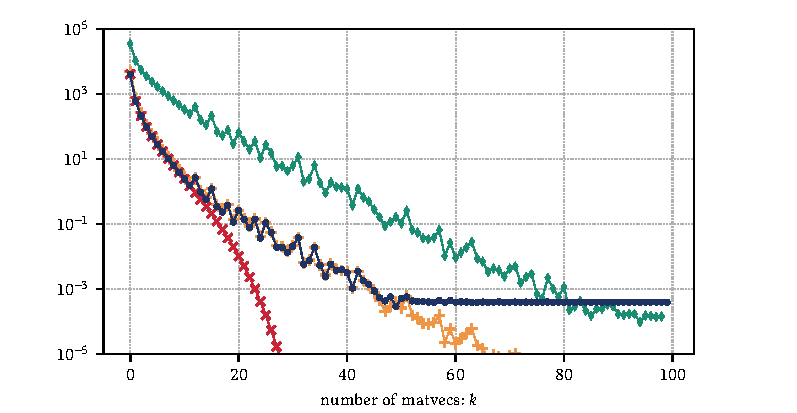
\includegraphics{imgs/ch8_CIF.pdf} 
    \end{center}
    \caption[{\( \vec{A}^2 \)-norm error bounds for \( f(x) = \sqrt{x} \) where \( \vec{A} \) has \( n=50 \) eigenvalues spaced according to the model problem with \( \rho = 0.8 \) and \( \kappa = 10^{3} \)}]{% 
        \( \vec{A}^2 \)-norm error bounds for \( f(x) = \sqrt{x} \) where \( \vec{A} \) has \( n=50 \) eigenvalues spaced according to the model problem with \( \rho = 0.8 \) and \( \kappa = 10^{3} \). We take \( \Gamma \) as a circular contour of radius \( \lmax \) centered at \( \lmax \) and \( w=0 \). Computations without reorthogonalization are run in single precision arithmetic, and error bounds are computed using \cref{thm:err_int} using the finite precision quantities.
    \hspace{.25em}\emph{Legend}:
    Lanczos-FA error with  
    ({\protect\raisebox{0mm}{\protect
\includegraphics[]{imgs/legend/l2.pdf}}}) and without 
    ({\protect\raisebox{0mm}{\protect
\includegraphics[]{imgs/legend/l1.pdf}}}) reorthogonalization, 
    a priori bounds with \( S = S_i = \mathcal{I} \)
    ({\protect\raisebox{0mm}{\protect
\includegraphics[]{imgs/legend/l3.pdf}}}), and
    a posteriori bounds obtained by using \cref{thm:err_int} with \( S = \mathcal{I} \)
    ({\protect\raisebox{0mm}{\protect
\includegraphics[]{imgs/legend/l4.pdf}}}).
    \hspace{.25em}\emph{Takeaway}: The bounds in finite precision arithmetic are accurate until near the ultimately attainable accuracy. 
    }
    \label{fig:ch8_CIF}
\end{figure}

Note that \( 1/(2\pi) \) times \cref{eqn:a_posteriori_fp} can be viewed as an upper bound of the ultimate obtainable  accuracy of Lanczos-FA in finite precision after convergence.
 If the inequalities do not introduce too much slack, this upper bound will also produce a reasonable estimate.
Since \( \| \vec{F} \| \) is small, one may simply ignore the contribution of \cref{eqn:a_posteriori_fp}, at least provided the Lanczos-FA error is not near the final accuracy.
Finally, we have worked in the \( (\vec{A}-w\vec{I})^2 \) norm as it simplifies some of the analysis, but in principle, a similar approach could be used with other norms.
This is straightforward, but would involve bounding something other than \( \|h_{w,z}\|_{S_0} \).

\subsection{Numerical experiment}



To illustrate the point of above analysis, we use a setup similar to what was used to produce \cref{fig:ch7_sqrt_Anorm}.
However, we now use the model problem and run Lanczos without reorthgonalization.
We use the \( \vec{T} \) produced in finite precision arithmetic in our computation of the error bounds from \cref{thm:err_int} and report the results in \cref{fig:ch8_CIF}.
Note that we use \cref{thm:err_int} and therefore do not account for the roundoff term analyzed above. 
However, since this term can be expected to be on the order of machine precision, the absence of this term in our computed bound does not significantly impact the bounds until near the ultimately attainable accuracy of Lanczos-FA. 
In other words, \cref{thm:err_int} still holds until the Lanczos-FA error is small.




\iffalse
\TODO{

\section{Lanczos-OR error}
\note{TODO if possible}
Recall that, in exact arithmetic,
\begin{align*}
    \| \err_k \|_{\tilde{N}\A}^2
    = \vec{e}_0^\cT \tilde{M}(\widehat{\vec{T}}) \tilde{N}(\widehat{\vec{T}})^{-1} \tilde{M}(\widehat{\vec{T}}) \vec{e}_0
    - \vec{e}_0^\cT [\tilde{M}(\widehat{\vec{T}})]_{:k,:k} ([\tilde{N}(\widehat{\vec{T}})]_{:k,:k})^{-1} [\tilde{M}(\widehat{\vec{T}})]_{:k,:k} \vec{e}_0.
\end{align*}

The expression on the right depends entirely on \( \Psi_{\vec{A},\vec{v}} \) and  the entries of \( \widehat{\vec{T}} \) required to compute \( [\tilde{M}(\widehat{\vec{T}})]_{:k,:k} \) and \( [\tilde{N}(\widehat{\vec{T}})]_{:k,:k} \).
Thus, we see that this expression will be nearly identical for the finite precision computaiton with \( \vec{A} \) and \( \vec{v} \) and the exact arithmetic computation with \( \bar{\vec{A}} \) and \( \bar{\vec{v}} \).

That the expressions on the left and right are near requires a bit more work.
In particular, we have made use of the identities \( \vec{Q}^\cT \tilde{M}(\vec{A}) \vec{v} = \tilde{M}(\widehat{\vec{T}}) \vec{e}_0 \) and \( \vec{Q}^\cT \tilde{N}\A \vec{Q} = [\tilde{N}(\widehat{\vec{T}})]_{:k,:k} \).
}

\fi
